\section*{Results and discussion}

Using data from a previous study of the corticospinal tract profile and ALS\cite{sarica2017corticospinal}, we tested the performance of AFQ-Insight in a classification setting. The previous study predicted ALS status with a mean accuracy of 80\% using a random forest algorithm based on a priori selection of features within the corticospinal tract. \adam{slight caveat here: not really a priori feature selection but rather a feature selection based on a mean decrease gini cutoff that seems a little bit like peaking. But anyway, I don't really want to recapitulate the entire Sarica paper here so perhaps saying a priori feature selection is a good shorthand}. AFQ-Insight delivers competitive predictive performance (mean 84\% accuracy, 0.93 ROC AUC) without the need for a priori feature engineering. The results of the classification prediction are shown in Fig~\ref{fig:class-results}.

\begin{figure}[!h]
    \centering
    %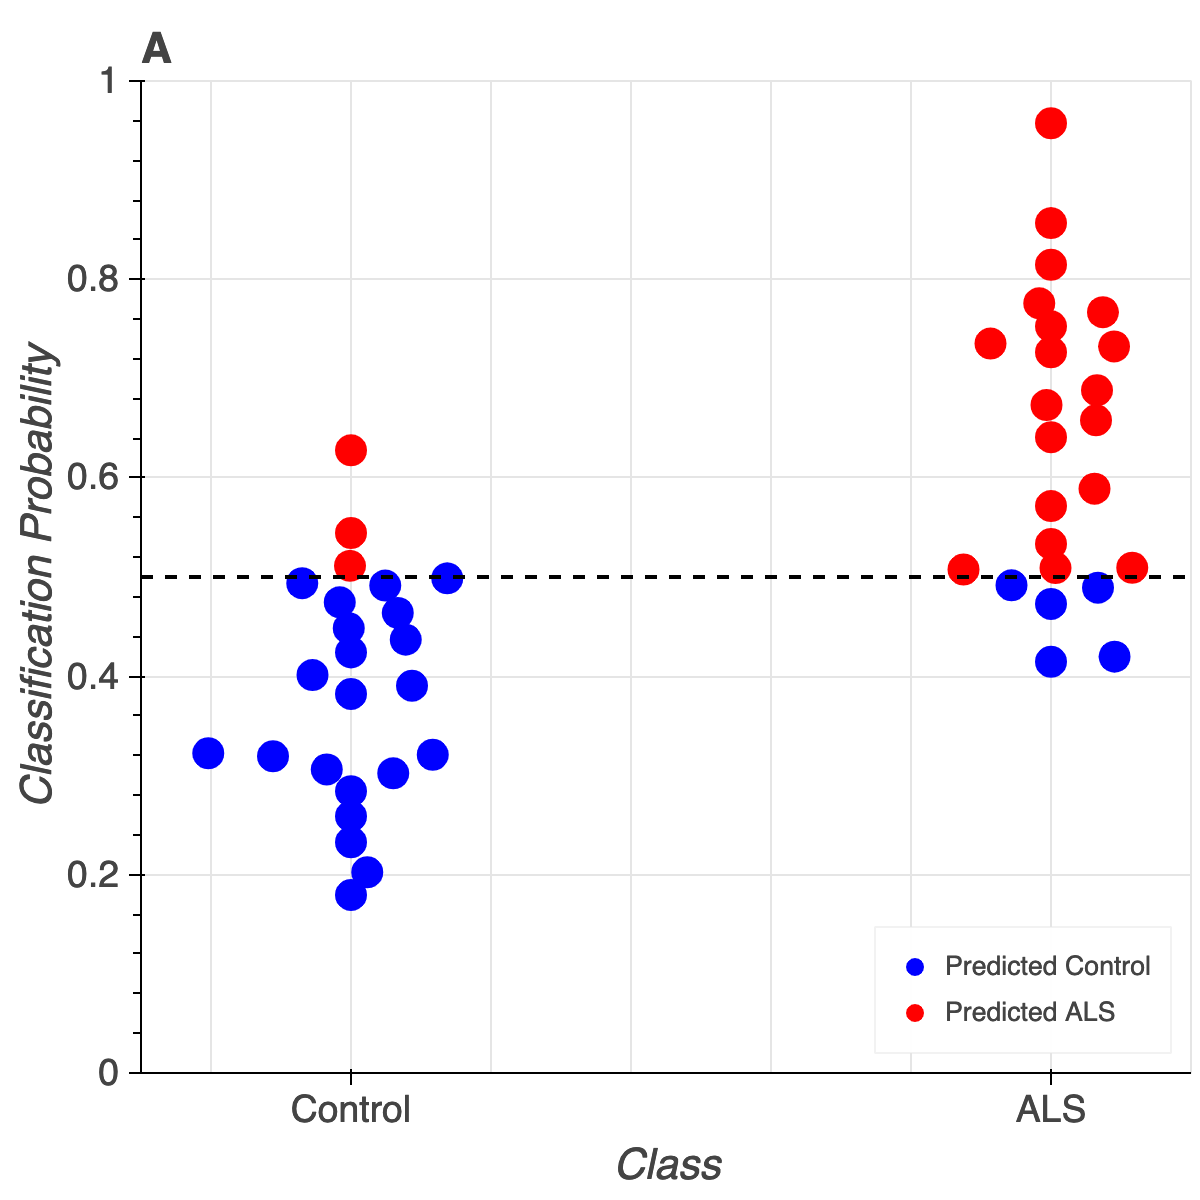
\includegraphics[width=0.65\textwidth]{classification_results.pdf}
    \caption{{\bf Prediction of ALS status.}
        Classification probabilities for each subject's ALS diagnosis. Controls are on the left while patients are on the right. Predicted controls are in blue and predicted patients are in red. Thus, false positive are represented as red dots on the left, while false negatives are represented as blue dots on the right. AFQ-Insight achieves 84\% accuracy with an ROC area under the curve of 0.93.
    }
    \label{fig:class-results}
\end{figure}

\begin{itemize}
  \item Classification
    \begin{itemize}
      \item Insert figure showing sparsity pattern
      \item Insert figure showing weights as they relate to tract differences visible in the browser
    \end{itemize}
\end{itemize}

In a regression setting, we attempted to accurately predict ``brain age''.

\begin{itemize}
  \item Regression
    \begin{itemize}
      \item Lifespan maturation age regression
      \item Insert figure showing sparsity pattern
      \item Insert figure showing weights as they relate to tract differences visible in the browser
    \end{itemize}
  \item Failures
    \begin{itemize}
      \item Hopefully, the failures are common to both regression
        and classification so we can include them here in there own
        subsection.
      \item Insert figure demonstrating failure cases
    \end{itemize}
\end{itemize}
